\documentclass[fleqn]{beamer}
\usepackage[english]{babel}

\usepackage{amsmath,amssymb}
\usepackage{graphicx}
\usepackage{tikz}
\usetikzlibrary{arrows.meta, positioning}

\graphicspath{{../../written_files/tesis_escrito/Figures/}}

\DeclareMathOperator*{\argmin}{arg\,min}
\DeclareMathOperator*{\argmax}{arg\,max}

% Beamer theme
\usetheme{ZMBZFMK}
\usefonttheme[onlysmall]{structurebold}
\mode<presentation>

\setlength{\jot}{0pt}

\AtBeginSection[]
{
  \begin{frame}
    \frametitle{Outline}
    \tableofcontents[currentsection]
  \end{frame}
}

\title{BASS as a Surrogate Model for Bayesian Optimization}
\author{Adrian Tame Jacobo}
\institute[Instituto Tecnológico Autónomo de México]{Thesis Defense}
\date{\today}

\begin{document}

\begin{frame}
  \titlepage
\end{frame}

% ---------------------------------------------------------------- %
\section{The Problem}

\begin{frame}
  \frametitle{Expensive black-box optimization}
  \begin{itemize}
    \item Many real objectives are \textbf{black boxes}: no formula, no gradients, only the ability to query $f(x)$ at a cost.
    \item The motivating instance: \textbf{hyperparameter tuning}. One evaluation equals one full training run, which can take hours.
    \item Goal: $x^* = \argmax_{\mathcal{X}} f(x)$ in as \textbf{few evaluations} as possible.
    \item Grid search and random search spend evaluations blindly; we want each query to be informed by everything seen so far.
  \end{itemize}
\end{frame}

\begin{frame}
  \frametitle{Bayesian optimization: the loop}
  \begin{enumerate}
    \item Fit a probabilistic \textbf{surrogate model} to the evaluations so far.
    \item Optimize an \textbf{acquisition function} over the surrogate to pick the most valuable next point.
    \item Pay for one true evaluation of $f$ there.
    \item Update the surrogate and repeat until the budget is spent.
  \end{enumerate}
  \vspace{2mm}
  The surrogate supplies two things at every candidate: a \textbf{prediction} and an \textbf{uncertainty}. The acquisition function trades them off (exploitation vs.\ exploration).
\end{frame}

\begin{frame}
  \frametitle{The surrogate is the method}
  \begin{itemize}
    \item The BO template is fixed machinery around one open slot: \textbf{which model fills the surrogate role}.
    \item The default, by a wide margin, is the \textbf{Gaussian process}: closed-form posterior mean and variance, exact interpolation, excellent with few points.
    \item But the GP's kernel measures \textbf{numeric distance} between inputs:
    \[ k(x, x') = \sigma_f^2 \exp\left( -\frac{(x - x')^2}{2\ell^2} \right) \]
    \item A categorical variable (model family, kernel choice, optimizer) has \textbf{no distance between its levels}. The standard GP cannot represent it natively.
  \end{itemize}
\end{frame}

\begin{frame}
  \frametitle{The categorical wall}
  \begin{itemize}
    \item Practical hyperparameter spaces mix continuous and \textbf{categorical} dimensions.
    \item Forcing categories into a GP means:
    \begin{itemize}
      \item integer encoding: fabricates an ordering that does not exist;
      \item one-hot encoding: distorts the geometry the kernel relies on;
      \item specialized kernels and embeddings: additional machinery, not the base model.
    \end{itemize}
    \item \textbf{Thesis question:} can a surrogate that treats categorical inputs natively, swapped into the same BO loop, reach the problems the GP cannot?
  \end{itemize}
\end{frame}

% ---------------------------------------------------------------- %
\section{The Proposal: BASS}

\begin{frame}
  \frametitle{Lineage: from trees to spline surfaces}
  \centering
  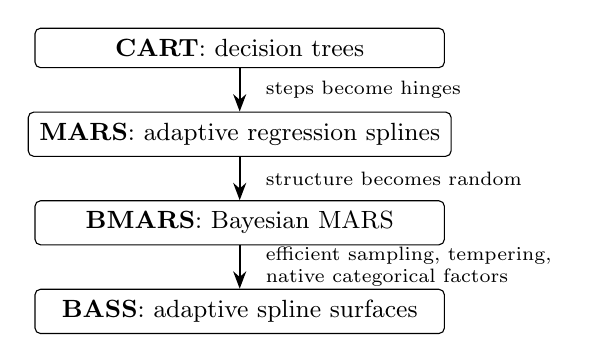
\begin{tikzpicture}[
      node distance=5.5mm,
      box/.style={draw, rounded corners=2pt, align=center, inner sep=4pt, minimum width=5.2cm, font=\small},
      lab/.style={align=left, font=\scriptsize},
      arr/.style={-{Stealth[length=2.2mm]}, thick}]
    \node[box] (cart) {\textbf{CART}: decision trees};
    \node[box, below=of cart] (mars) {\textbf{MARS}: adaptive regression splines};
    \node[box, below=of mars] (bmars) {\textbf{BMARS}: Bayesian MARS};
    \node[box, below=of bmars] (bass) {\textbf{BASS}: adaptive spline surfaces};
    \draw[arr] (cart) -- (mars) node[midway, right=2mm, lab] {steps become hinges};
    \draw[arr] (mars) -- (bmars) node[midway, right=2mm, lab] {structure becomes random};
    \draw[arr] (bmars) -- (bass) node[midway, right=2mm, lab] {efficient sampling, tempering,\\native categorical factors};
  \end{tikzpicture}
\end{frame}

\begin{frame}
  \frametitle{The BASS model}
  \begin{align*}
    y_i &= f(\boldsymbol{x}_i) + \epsilon_i, \qquad \epsilon_i \sim \mathcal{N}(0, \sigma^2) \\
    f(\boldsymbol{x}) &= a_0 + \sum_{m=1}^{M} a_m B_m(\boldsymbol{x}) \\
    B_m(\boldsymbol{x}) &= \prod_{k=1}^{K_m} g_{km} \left[ s_{km}\left(\boldsymbol{x}_{v_{km}} - t_{km}\right) \right]^\alpha_+
  \end{align*}
  \begin{itemize}
    \item A sum of $M$ basis functions, each a product of hinge factors: signs $s_{km}$, knots $t_{km}$, selected variables $v_{km}$.
    \item Everything MARS fixes greedily is a \textbf{random quantity} here: $M$, the structure of every basis, the coefficients, and $\sigma^2$ all carry priors.
  \end{itemize}
\end{frame}

\begin{frame}
  \frametitle{Where Bayes enters}
  \begin{itemize}
    \item Priors: $M \sim \text{Poisson}(\lambda)$, coefficients under a Zellner $g$-prior, $\sigma^2$ inverse-gamma, uniform structural priors on knots, signs, and variables.
    \item The posterior over \textbf{entire model configurations} is sampled by \textbf{reversible-jump MCMC}: birth, death, and change moves over basis functions.
    \item The fitted object is not one surface but a \textbf{collection of posterior draws over surfaces}.
    \item Parallel tempering keeps the sampler exploring rather than stuck.
  \end{itemize}
\end{frame}

\begin{frame}
  \frametitle{Categorical inputs, natively}
  \begin{itemize}
    \item For a continuous variable, a factor of $B_m$ is a hinge: a slope change at a numeric knot.
    \item For a categorical variable, the factor becomes an \textbf{indicator on a subset of levels}:
    \[ \boldsymbol{1}\left[ \boldsymbol{x}_{v_{km}} \in S_{km} \right], \qquad S_{km} \subseteq \mathcal{L} \]
    \item The subset $S_{km}$ plays the role of the knot, and it is just another random quantity the sampler explores.
    \item Continuous and categorical factors combine in the same product, so \textbf{mixed interactions} are represented directly. No encodings.
  \end{itemize}
\end{frame}

\begin{frame}
  \frametitle{Uncertainty without a closed form}
  \begin{itemize}
    \item A GP hands the acquisition function a closed-form variance. BASS does not, but it does not need to.
    \item Evaluating the $S$ posterior draws at a candidate $\boldsymbol{x}$ gives a sample from the posterior predictive of $f(\boldsymbol{x})$.
    \item Monte Carlo Expected Improvement, with $f_{\text{best}}$ the incumbent:
    \[ \widehat{\mathrm{EI}}(\boldsymbol{x}) = \frac{1}{S} \sum_{s=1}^{S} \max\left(0,\; f_{\text{best}} - f^{(s)}(\boldsymbol{x})\right) \]
    \item No exploration weight to tune: the spread of the draws supplies the balance automatically.
  \end{itemize}
\end{frame}

% ---------------------------------------------------------------- %
\section{Experimental Design}

\begin{frame}
  \frametitle{One moving part: the surrogate}
  \begin{itemize}
    \item Methods: \textbf{BASS-BO}, \textbf{GP-BO}, \textbf{TPE} (Optuna), \textbf{Random Search}.
    \item Shared across all methods, per seed: the same LHS initial design, the same candidate generator, the same parameter-free Expected Improvement, the same budget.
    \item 25 seeds per benchmark; paired per-seed statistics against Random Search (win/tie/loss and Wilcoxon signed-rank).
    \item Benchmarks in three regimes: \textbf{continuous} (Branin, Rastrigin, a non-smooth synthetic), \textbf{purely categorical} (Cat-Ackley at three sizes), and \textbf{mixed} (Func-2C, Func-3C).
  \end{itemize}
\end{frame}

\begin{frame}
  \frametitle{Why shared machinery matters}
  \begin{itemize}
    \item Oracle audits (acquisition replaced by the true objective) showed the \textbf{candidate generator alone} can decide whether any surrogate reaches the optimum of a mixed benchmark.
    \item Before combination-level duplicate handling, roughly two thirds of a small categorical budget was silently re-spent on known configurations.
    \item Both effects are invisible in a convergence plot, and both would have been misread as surrogate differences.
    \item Consequence: surrogate comparisons in mixed and categorical spaces are only meaningful when the search machinery is \textbf{shared, categorical-aware, and audited}.
  \end{itemize}
\end{frame}

% ---------------------------------------------------------------- %
\section{Results}

\begin{frame}
  \frametitle{Continuous: the GP earns its default}
  \centering
  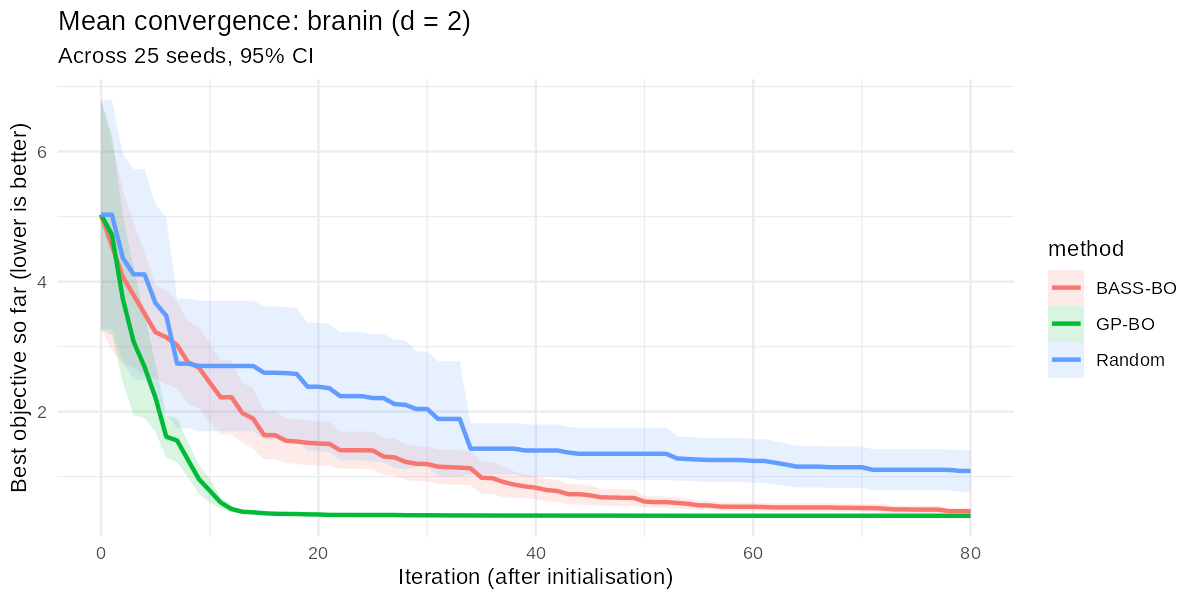
\includegraphics[width=0.72\textwidth]{conv_branin.png}
  \begin{itemize}
    \item Branin: GP-BO beats BASS-BO on \textbf{25 of 25} paired seeds; Rastrigin: 21 of 25.
    \item Both surrogate methods clear Random Search on every continuous benchmark; on the non-smooth synthetic surface the two surrogates tie.
  \end{itemize}
\end{frame}

\begin{frame}
  \frametitle{Categorical: capability demonstrated}
  \centering
  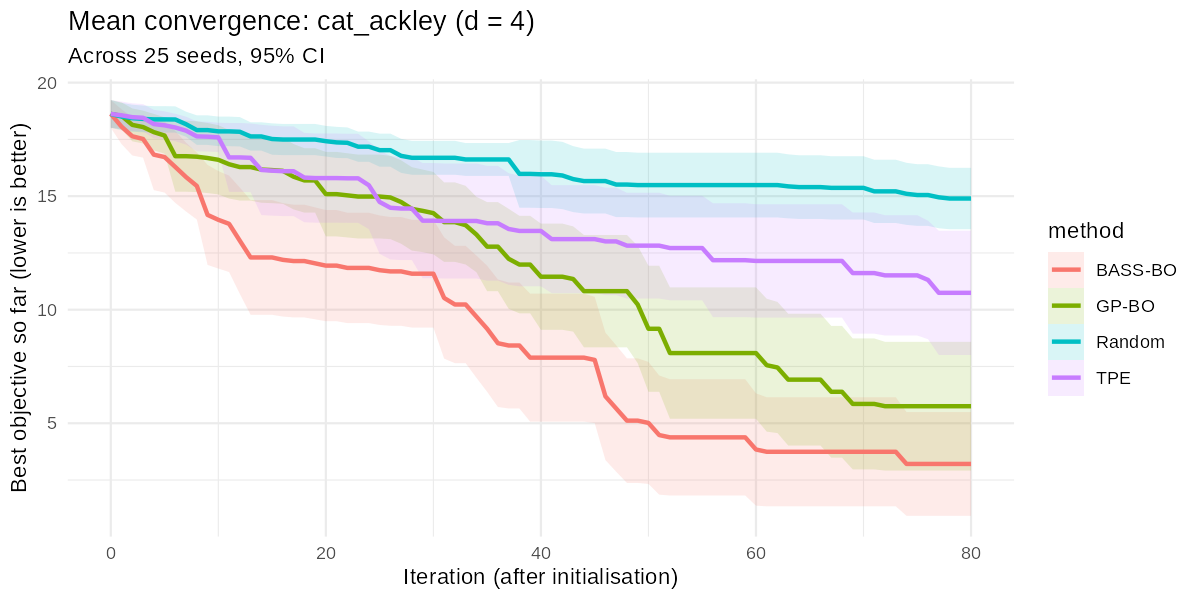
\includegraphics[width=0.72\textwidth]{conv_cat_ackley_medium.png}
  \begin{itemize}
    \item Easy instance: BASS-BO solves \textbf{25/25} seeds (GP-BO 25, TPE 20, RS 17).
    \item Medium: BASS-BO \textbf{19/25} vs.\ GP-BO 15, TPE 7, Random Search 1.
    \item Hard: BASS-BO beats Random Search on \textbf{all 25} paired seeds and never loses a seed to TPE at any size.
  \end{itemize}
\end{frame}

\begin{frame}
  \frametitle{Mixed spaces: an honest negative}
  \centering
  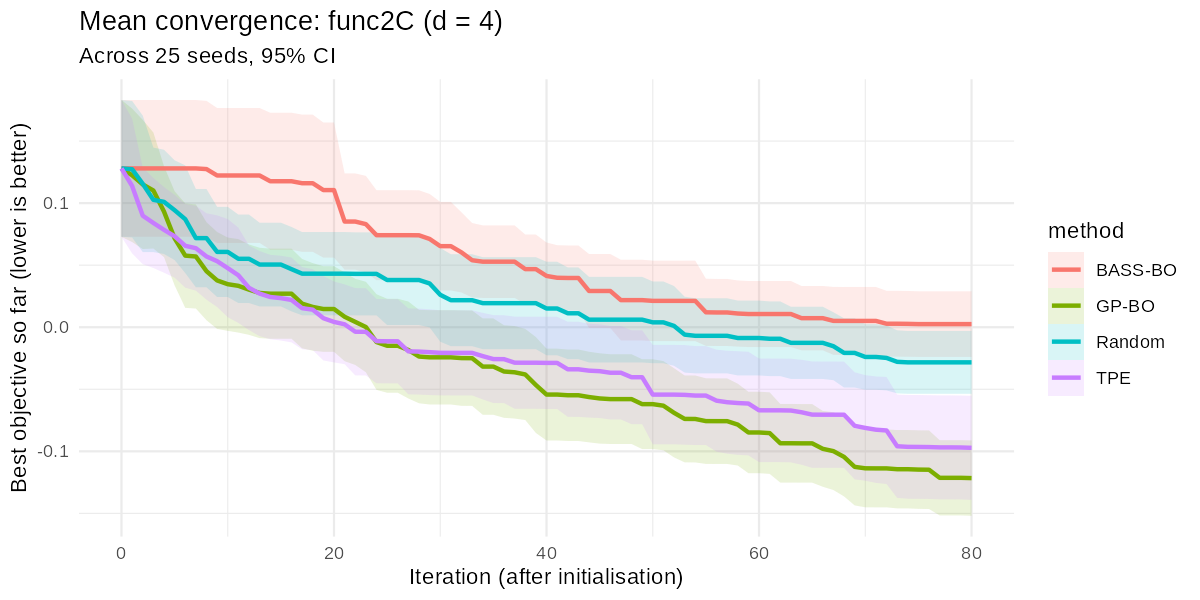
\includegraphics[width=0.72\textwidth]{conv_func2C.png}
  \begin{itemize}
    \item On Func-2C and Func-3C, BASS-BO \textbf{loses to Random Search} under the paired test (5W-18L and 8W-14L, both significant at 5\%).
    \item GP-BO and TPE beat Random Search comfortably on the same seeds.
    \item Reported with the same prominence as the positive results: in its present form BASS-BO is not recommendable for mixed spaces.
  \end{itemize}
\end{frame}

\begin{frame}
  \frametitle{The regime map}
  \begin{itemize}
    \item \textbf{Smooth, low-dimensional, continuous:} GP-BO decisively; BASS-BO a clear-but-second improvement over Random Search.
    \item \textbf{Purely categorical:} BASS-BO solves what the budget makes solvable, outperforms Random Search and TPE, and matches a GP given the same categorical-aware machinery.
    \item \textbf{Mixed continuous-categorical:} negative result for BASS-BO as implemented; GP-BO and TPE are the working choices.
    \item The structural argument alone would have predicted more; the measured map is sharper and more honest.
  \end{itemize}
\end{frame}

% ---------------------------------------------------------------- %
\section{Conclusions}

\begin{frame}
  \frametitle{Contributions}
  \begin{itemize}
    \item \textbf{Empirical:} BASS earns a place as a surrogate for purely categorical search spaces, evaluated under paired, seed-matched statistics.
    \item \textbf{Methodological:} a reproducible pipeline where the surrogate is the only moving part, and direct evidence of how much apparent surrogate difference actually lives in the search machinery.
    \item \textbf{Honest reporting:} the mixed-space failure is documented and analyzed, not obscured.
  \end{itemize}
\end{frame}

\begin{frame}
  \frametitle{Future work}
  \begin{itemize}
    \item Richer categorical proposals: correlated multi-coordinate moves informed by the surrogate's own level effects.
    \item Real mixed hyperparameter-tuning tasks, beyond synthetic benchmarks.
    \item Broader continuous suites: multimodal, higher-dimensional, noisy objectives.
    \item The machinery-confound audit as a general diagnostic, developed separately.
  \end{itemize}
\end{frame}

\begin{frame}
  \frametitle{Disclosure: AI use in this thesis}
  \begin{itemize}
    \item Development used Anthropic's Claude Code in author-driven sessions: the author directs, decides, and approves; the assistant drafts, implements, and verifies under that direction.
    \item Every AI-assisted change entered the repository through a pull request reviewed by the author; no content reached the thesis without that review.
    \item Scope: benchmarking infrastructure, figure generation, editing passes over the manuscript, and the systematic processing of the advisor's corrections.
    \item The full record lives in the repository: \texttt{docs/AI\_DISCLOSURE.md}.
  \end{itemize}
\end{frame}

\begin{frame}
  \begin{center}
    {\Large Thank you.} \\[4mm]
    Questions welcome.
  \end{center}
\end{frame}

\end{document}
